\chapter{Introducción al Machine Learning}\label{cap:ml}

El Machine Learning o Aprendizaje Automático es la rama de las Ciencias de la Computación, y en particular, de la Inteligencia de la Artificial que se encarga del reconocimiento de patrones y de la teoría computacional del aprendizaje~\cite{machinelearningbritannica}. El machine learning se basa en la construcción de modelos que permitan aprender y hacer predicciones sobre unos datos, de forma automática, es decir, sin intervención humana~\cite{24218}.\\

El machine learning permite resolver infinidad de problemas que se pueden clasificar de la siguiente manera:

\begin{itemize}
	\item \textbf{Clasificación:} las entradas son divididas entre dos o más clases y el modelo debe aprender a asignar a cada entrada una de las clases.~\cite[pág 9]{Marsland:2009:MLA:1571643}\\
	
	Un ejemplo clásico de problema de clasificación es el filtro de spam: el modelo debe ser capaz de identificar un correo electrónico como ``spam'' o ``no spam'', es decir, éstas serán las clases en las que se deberán dividir las entradas (por ejemplo, número de apariciones o frecuencia de distintas palabras en el correo) para identificar el spam.
	
	\item \textbf{Regresión:} las salidas son continuas. En contraposición con la clasificación, la regresión tiene una salida continua, es decir, puede tomar todos los valores reales o un intervalo de ellos.~\cite[pág 8]{Marsland:2009:MLA:1571643}\\
	
	Por ejemplo, el valor de las acciones de una determinada empresa a lo largo del tiempo es un ejemplo de regresión, ya que el valor de las acciones pueden tomar cualquier valor en el intervalo $[0, \infty)$.
	
	\item \textbf{Clustering:} un conjunto de entrada se divide en grupos (los grupos no están fijados de antemano).~\cite[pág 195]{Marsland:2009:MLA:1571643}
	
	Un ejemplo clásico es la segmentación del mercado, es decir, encontrar grupos con similares características de una población para ofrecer ofertas personalizadas.
	
	\item \textbf{Reducción de dimensionalidad:} simplifica las entradas por medio de una función a un espacio de dimensión inferior.~\cite[pág 221]{Marsland:2009:MLA:1571643}   
\end{itemize}

En el machine learning puede clasificarse por tipo de aprendizaje:

\begin{itemize}
	\item \textbf{Aprendizaje supervisado:} consiste en construir un modelo a partir de un conjunto de entrenamiento que contiene los datos de entrada y la salida (o etiqueta) esperada. El algoritmo produce un modelo para inferir la salida de nuevos ejemplos ~\cite[pág~ 7]{Marsland:2009:MLA:1571643}.
	
	En este tipo de aprendizaje se incluye la tarea de clasificación y la regresión.
	
	\item \textbf{Aprendizaje no supervisado:} en este caso no existen etiquetas predefinidas de antemano, y se trata de encontrar una función que describa la estructura oculta de los datos~\cite[pág 195]{Marsland:2009:MLA:1571643}.\\
	
	En este tipo de aprendizaje se incluye el clustering.
	
	\item \textbf{Aprendizaje por refuerzo:} un ordenador interactúa con un entorno dinámico para conseguir una determinada recompensa, sin que un nadie le diga como de lejos está de conseguirla~\cite[pág 4]{Sutton:1998:IRL:551283}.  
\end{itemize}

A continuación veremos cada uno de estos tipos con más profundidad.

\section{Aprendizaje supervisado}

En el aprendizaje supervisado existe un \textit{conjunto de entrenamiento} que consiste en un conjunto de datos de entrada junto con su correspondiente salida, que es la respuesta que un algoritmo de machine learning debería producir para esa entrada. Normalmente se representa como un vector $(\mathbf{x}, \mathbf{y})$, donde $\mathbf{x} = (x_1,...,x_n)$ son las entradas y $\mathbf{y} = (y_1,...,y_n)$, las salidas.\\

Una característica importante de los algoritmos de machine learning es la capacidad de generalización: el algoritmo debería producir salidas \textit{sensatas} para entradas que no se introdujeron en el entrenamiento. También es importante que el algoritmo pueda tratar con el ruido, es decir, con las imprecisiones que se  obtienen al medir cualquier variable del mundo real.\\

Dentro de este tipo de aprendizaje tenemos varios tipos de problemas, entre los que se encuentran la clasificación y la regresión.

\paragraph{Clasificación}
El problema de clasificación consiste en tomar las entradas y decidir a cuál de las $n$ clases pertenece cada entrada, basado en el entrenamiento con ejemplares de cada clase. Un punto clave en el problema de clasificación es que es discreto, es decir, cada ejemplo pertenece a una sola de las clases y el conjunto de clases cubre por completo el espacio de salida.

\begin{ejemplo}
Consideremos la clasificación de un correo electrónico como ``spam'' o ``no spam''. En este caso el conjunto de clases vendría dado por $C = \{ \text{spam}, \text{no spam} \}$. Las entradas podrían venir dadas, por ejemplo, por la frecuencia de aparición de distintas palabras claves del correo electrónico y la salida vendría dada por una de las clases (spam, no spam). 
\end{ejemplo}

\paragraph{Regresión}
El problema de regresión consiste en obtener un valor de salida a partir de las entradas. En contraposición con el problema de clasificación, las salidas toman valores sobre un intervalo continuo.

\begin{ejemplo}
Supongamos que queremos estimar el valor de las acciones de una determinada empresa a partir de una serie de variables como el número de empleados, los ingresos, etc. En este caso estamos ante un problema de regresión ya que la variable salida (valor de las acciones) toma un valor continuo en el intervalo $[0,\infty)$.  
\end{ejemplo}

Existen diferentes tipos de regresión, aunque solo nos centraremos en la regresión lineal.

\subparagraph{Regresión lineal}
La regresión lineal viene dada por el modelo~\cite[pág 255]{mathews2004numerical}

\begin{equation}
y_i = \alpha_1 x_{i1} + \dots + \alpha_p x_{ip} + \alpha_0, \quad i = 1,...,n
\end{equation}

donde $y_i$ es la variable salida, $x_{i}$ es la variable de entrada, $n$ es el número de observaciones y $p$ es el número de variables de entrada.\\

El método de mínimos cuadrados nos garantiza que los parámetros $\alpha_i$ que minimizan el error cuadrático\footnote{El error cuadrático viene dado por \begin{equation}
\mathrm{EC} = \sum_{i=1}^{n} (\hat{y}_i - y_i) 
\end{equation} 
donde $\hat{y}$ es el valor ajustado de la variable salida y $y$ es el valor real de la variable salida} vienen dados por

\begin{equation}
\boldsymbol{\alpha} = (\mathbf{X}^T \mathbf{X})^{-1} \mathbf{X}^T \mathbf{y}.
\end{equation}

donde 

\begin{equation*}
\mathbf{\alpha} = (\alpha_1,...,\alpha_n)^T,
\end{equation*}

\begin{equation*}
\mathbf{y} = (y_1,...,y_n)^T,
\end{equation*}

\begin{equation*}
\mathbf{X} = \left(\begin{matrix}{ccc}
x_{11} & ... & x_{1p} \\
x_{21} & ... & x_{2p} \\
\vdots & \ddots & \vdots \\
x_{n1} & \dots & x_{np}
\end{matrix}\right)
\end{equation*}

En particular, en el caso bidimensional el modelo viene dado por

\begin{equation}
y = \alpha_1 x + \alpha_0.
\end{equation}

Se tiene que $\alpha_0$ y $\alpha_1$ vienen dados por este sistema de ecuaciones lineales:

\begin{equation}
\begin{cases}
\begin{array}{ccccc}
\left(\displaystyle\sum_{i=1}^{n} x_i^2\right) \alpha_1 & + & \left(\displaystyle\sum_{i=1}^{n} x_i\right) \alpha_0 & = & \displaystyle \sum_{i=1}^{n} x_i y_i \\
 \left(\displaystyle \sum_{i=1}^{n} x_i\right) \alpha_1 & + & n \alpha_0 & = & \displaystyle \sum_{i=1}^{n} y_i
\end{array}
\end{cases}
\end{equation}

\begin{ejemplo}
	Supongamos que disponemos de los datos de la Tabla~\ref{tbl:regresion_lineal} y queremos ajustar un modelo lineal de la forma $y = \alpha_1 x + \alpha_0$.\\
	
	De acuerdo a lo anterior, los valores $\alpha_0$ y $\alpha_1$ que minimizan el error cuadrático son las soluciones del sistema
	
	\begin{equation*}
	\begin{cases}
	\begin{array}{ccccc}
	92 \alpha_1 & + & 20 \alpha_0 & = & 25 \\
	20 \alpha_1 & + &  8 \alpha_0 & = & 37
	\end{array}
	\end{cases}
	\end{equation*}
	
	Resolviendo el sistema lineal, se tiene que,
	
	\begin{eqnarray*}
	\alpha_1 \approx -1.607 \\
	\alpha_0 \approx  8.642
	\end{eqnarray*}
	
	Por tanto, $y = -1.607x + 8.642$.
	
	Si quisiéramos predecir el valor para $x=7$, tendríamos que $y = -1.607\cdot 7 + 8.642 = -2.607$.
	
	\begin{table}[htbp!]
		\centering
		\caption{Datos para regresión lineal}
		\label{tbl:regresion_lineal}
		\begin{tabular}{@{}lllllllll@{}}
			\toprule
			$x$ & -1 & 0 & 1 & 2 & 3 & 4 & 5 & 6  \\ \midrule
			$y$ & 10 & 9 & 7 & 5 & 4 & 3 & 0 & -1 \\ \bottomrule
		\end{tabular}
	\end{table}
	
\end{ejemplo}

Es importante notar que este método permite ajustar modelos que, en principio, no son lineales como, por ejemplo, 

\[ y = ax^m \]

Este modelo no puede ajustarse como regresión lineal, pero se pueden linealizar las variables $x$, $y$ para convertirlo en un modelo lineal~\cite[pág 257]{mathews2004numerical}.\\

Tomando logaritmos a ambos lados de la igualdad,

\[ \log y = \log(ax^m)  = \log a + m \log x \]

Haciendo $Y = \log y$, $X = \log x$, $\alpha_1 = \log a$ y $m = \alpha_0$, tenemos un modelo lineal.\\

En la Tabla~\ref{tbl:linealizacion} se pueden encontrar cómo linealizar otros modelos de forma que la regresión lineal resuelve muchos otros casos.\\

Otros tipos de regresión se pueden encontrar en ~\cite{citeulike:12658828}, como la regresión logística o los modelos generales lineales, entre otros.

\begin{table}[htbp!]
	\centering
	\caption{Linealización de distintos modelos}
	\label{tbl:linealizacion}
	\begin{tabular}{@{}ccc@{}}
		\toprule
		$y = f(x)$                             & \begin{tabular}[c]{@{}c@{}}Forma linealizada\\ $y = \alpha_1 x + \alpha_0$\end{tabular} & \begin{tabular}[c]{@{}c@{}}Cambio de variables\\ y constantes\end{tabular} \\ \midrule
		$y = \dfrac{\alpha_1}{x} + \alpha_0$   & $y = \alpha_1 \dfrac{1}{x} + \alpha_0$                                                  & $X=\dfrac{1}{x}$; $Y=y$                                                    \\
		$y = \dfrac{1}{\alpha_1 x + \alpha_0}$ & $\dfrac{1}{y} = \alpha_1 x + \alpha_0$                                                  & $Y=\dfrac{1}{y}$; $X=x$                                                    \\
		$y = \alpha_1 \log x + \alpha_0$       & $y = \alpha_1 \log x + \alpha_0$                                                        & $Y = y$; $X = \log x$                                                      \\
		$y = \alpha_1 e^{\alpha_0 x}$          & $\log y = \log \alpha_1 + \alpha_2 \log x$                                              & $Y = \log y$; $X = \log x$; $\alpha_1 = \log \alpha_1$                     \\
		$y = (\alpha_0 + \alpha_1 x)^2$        & $\sqrt{y} = \alpha_0 + \alpha_1 x$                                                      & $Y = \sqrt{y}$; $X=x$                                                      \\ \bottomrule
	\end{tabular}
\end{table} 

\subsection{El proceso de Machine Learning supervisado}

El proceso general para resolver un problema usando aprendizaje supervisado consiste en los siguientes pasos~\cite{Marsland:2009:MLA:1571643}:

\begin{enumerate}
	\item \textbf{Obtención de datos y preparación:} consiste en obtener y preparar los datos que se usarán para obtener un modelo de machine learning adecuado para los datos. Consiste en obtener unos datos que sean relevantes, tarea que es difícil cuando se dispone de una cantidad de datos muy grande y que contiene outliers y datos faltantes.
	
	\item \textbf{Selección de características:} consiste en la identificación de características que sean más útiles para el problema en cuestión.
	
	\item \textbf{Elección del algoritmo:} dado el conjunto de datos, consiste en elegir uno o varios algoritmos adecuados que permita resolver el problema de manera satisfactoria.
	
	\item \textbf{Selección del modelo y sus parámetros:} la mayoría de los algoritmos de Machine Learning tienen parámetros que deben ser fijados manualmente, o que requieren experimentación para obtener valores adecuados.
	
	\item \textbf{Entrenamiento:} dado el conjunto de datos, el algoritmo y los parámetros, el entrenamiento deberá construir un modelo a partir de los datos para predecir las salidas de nuevos datos.
	
	\item \textbf{Evaluación:} antes de que el sistema sea desplegado, necesita ser probado y evaluado con datos con los que no ha sido entrenado. A veces, incluye una comparación con expertos humanos en el campo y la selección de métricas apropiadas para esa comparación.    
\end{enumerate}

De los 6 puntos anteriores, nos centraremos en la elección del algoritmo. De entre todos los algoritmos entraremos en detalle de las redes neuronales, los Support Vector Machine (SVM) y los árboles de decisión, por ser ampliamente estudiados y están basados en conceptos diferentes. Las redes neuronales se basan en el funcionamiento biológico de las neuronas, los SVM en elevar la dimensión y el uso de kernels, y los árboles de decisión que se basan en obtener reglas fácilmente entendibles por humanos.

\subsection{Redes neuronales}

Las redes neuronales están basadas en el modo que funcionan las neuronas en el cerebro. La operación general de la misma es transmitir químicos dentro del fluido del cerebro para aumentar o disminuir el potencial eléctrico dentro del cuerpo de la neurona. Si el potencial de la neurona alcanza algún determinado umbral, la neurona se activa y un pulso de duración fija se envía al axón. El axón se divide en conexiones a muchas otras neuronas, conectando a estas neuronas en una sinapsis~\cite[pág 11]{Marsland:2009:MLA:1571643}.\\

\begin{figure}[tbph!]
\centering
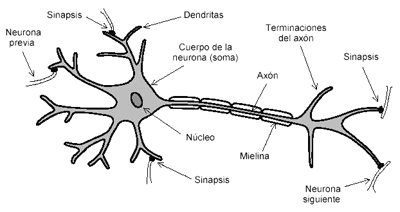
\includegraphics[width=0.7\linewidth]{imagenes/neurona.png}
\caption{Estructura de una neurona}
\label{fig:neurona}
\end{figure}

En 1943, McCulloch y Pitts propusieron un modelo matemático simplificado del funcionamiento de una neurona con las siguientes características (Figura~\ref{fig:mccullochpitts}):

\begin{figure}[htbp!]
\centering
\neuronaMcCullochPitts
\caption{Neurona de McCulloch y Pitts}
\label{fig:mccullochpitts}
\end{figure}

\begin{itemize}
	\item Un conjunto de pesos $w_i$ que corresponden con la sinapsis.
	\item Un sumador $\Sigma$ que suma las señales entrantes (equivalente a la membrana de la célula que recoge la carga eléctrica)
	\item Una función de activación $g$ que decide si la membrana se activa o no para las entradas actuales. 
\end{itemize} 

Llamaremos $h$ a a la suma de las entradas multiplicadas por los pesos.\\

Es decir $h$ es,

\begin{equation}
h = \sum_{i=1}^{n} w_i x_i.
\end{equation}

Si $h > \theta$ (valor fijado), la neurona se activará. Matemáticamente,

\begin{equation}
y = g(h) =
\begin{cases}
1 & \text{ si } h > \theta \\
0 & \text{ si } h  \leq \theta
\end{cases}
\end{equation}

Un problema obvio de la neurona de McCulloch y Pitts es que sólo puede activarse o no hacerlo, por lo que no puede aprender. Para ello, necesitamos poner neuronas juntas formando una red neuronal~\cite[pág 11]{Marsland:2009:MLA:1571643}.\\

El \textbf{perceptrón} es la red neuronal más sencilla, ya que no es más que una colección de neuronas de MacCulloch y Pitts (Figura~\ref{fig:perceptron}).

\begin{figure}[htbp!]
	\centering
	\perceptron
	\caption{Perceptrón}
	\label{fig:perceptron}
\end{figure}

A la izquierda se sitúan las entradas y a la derecha se muestran las neuronas. Éstas son completamente indepedendientes unas de otras: no importa qué estén haciendo las otras neuronas, la neurona se activará multiplicando sus pesos por las entradas, sumando el resultado y comparando el resultado con su umbral, sin importar lo que estén haciendo las demás neuronas.\\

Una limitación importante del perceptrón es que sólo es capaz de clasificar conjuntos linealmente separables\footnote{Un conjunto es linealmente separable si existe un hiperplano que separe dos clases.}. Novikoff probó que el algoritmo de aprendizaje de un perceptrón converge en un número finito de iteraciones si los datos son linealmente separables~\cite{Novikoff:1962}.\\

\begin{figure}[htbp!]
	\begin{center}
		\begin{subfigure}[b]{.40\textwidth}
			\centering
			\linealmenteseparable
			\caption{Linealmente separable}
		\end{subfigure}
		\begin{subfigure}[b]{.40\textwidth}
			\centering
			\nolinealmenteseparable
			\caption{No linealmente separable}
		\end{subfigure}
		
	\end{center}
	\caption{Conjuntos linealmente separables y no separables}
	\label{fig:linealmente_separable}
\end{figure}

Un ejemplo clásico que no puede aprender un perceptrón es la función XOR: $\{0,1\} \times \{0,1\} \to \{0,1\}$, que se define como se ve en la Tabla~\ref{tbl:xor}.\\


\begin{table}[htbp!]
	\centering
	\caption{Definición de la función XOR}
	\label{tbl:xor}
	\begin{tabular}{@{}ccc@{}}
		\toprule
		x & y & XOR \\ \midrule
		0 & 0 & 0   \\
		0 & 1 & 1   \\
		1 & 0 & 1   \\
		1 & 1 & 0   \\ \bottomrule
	\end{tabular}
\end{table}

Si representamos estos puntos en el plano xy (Figura~\ref{fig:xor}), veremos que no podemos encontrar ningún hiperplano (en este caso, recta) que divida a las dos clases.\\

\begin{figure}[htbp!]
	\centering
	\xor
	\caption{Función XOR}
	\label{fig:xor}
\end{figure}

Para suplir la limitación anterior, nació el perceptrón multicapa, que consiste en múltiples capas de neuronas (Figura~\ref{fig:perceptron_multicapa}).

\begin{figure}[htbp!]
	\centering
	\perceptronmulticapa
	\caption{Perceptrón multicapa}
	\label{fig:perceptron_multicapa}
\end{figure}

El teorema de aproximación universal establece que un perceptrón multicapa con una capa oculta puede aproximar funciones continuas sobre conjuntos compactos de $\R^n$ \cite{Cybenko1989}.\\

Una descripción de los algoritmos del perceptrón multicapa se pueden encontrar en~\cite{Bishop:2006:PRM:1162264,Marsland:2009:MLA:1571643, Murphy:2012:MLP:2380985}.

\subsection{Support Vector Machine}
Los Support Vector Machine (SVM) son uno de los algoritmos más populares en machine learning. Fueron introducidos en 1992 por Vapnik~\cite{Cortes:1995:SN:218919.218929} y se han empleado en multitud de aplicaciones desde entonces, debido principalmente a que consigue una gran tasa de clasificación en conjuntos de datos con tamaño razonable. Los SVM no funcionan bien en conjuntos de datos muy grande, ya que los cálculos no escalan bien con el número de datos, y se vuelve computacionalmente muy costoso~\cite[pág 119]{Marsland:2009:MLA:1571643}.\\

La Figura~\ref{fig:clasificador} muestra una clasificación con tres posibles clasificadores lineales. Las tres rectas dividen de forma ``correcta'' ambas clases, por lo que el perceptrón pararía si encontrara cualquiera de ellas, teniendo varias soluciones.\\

\begin{figure}[htbp!]
	\centering
	\clasificador
	\caption{Distintos clasificadores lineales}
	\label{fig:clasificador}
\end{figure}

Los SVM se basan el concepto de margen (Figura~\ref{fig:margen}), que no es nada más que la región más grande que podemos separar las clases sin que haya puntos dentro, donde la caja se hace con dos líneas paralelas al clasificador lineal. El clasificador que tenga mayor margen se llamará clasificador con mayor margen. Los puntos de cada clase que están más cerca de la recta reciben el nombre de vectores de soporte (support vectors).\\

 \begin{figure}[htbp!]
	\centering
	\margen
 	\caption{Margen en SVM}
 	\label{fig:margen}
 \end{figure} 
 
 Se puede demostrar~\cite{Bishop:2006:PRM:1162264,Marsland:2009:MLA:1571643} que el problema anterior se puede plantear como un problema de programación cuadrática con la siguiente estructura:
 
 \begin{align}
 \min & \ \ \ \dfrac{1}{2}\mathbf{w}^T \mathbf{w}\\
 \text{s.a. } & \ \ \ y_i (\mathbf{w}^T x_i + b) \geq 1 \ \forall i = 1,\dots, n
 \end{align}
 
 donde $\mathbf{x}$ es el vector de entradas, $\mathbf{w}$ es un vector perpendicular al hiperplano clasificador, $b$ es una constante y $y_i$ es el valor de la salida i-ésima que puede  tomar dos valores $\{-1,1\}$.\\
 
 Otro concepto fundamental en SVM es el de \textbf{kernel}, que consiste en modificar las variables de alguna forma que se puedan separar los datos (Figura~\ref{fig:kernel}).\\
 
\begin{figure}[htbp!]
	\centering
	\kernel
	\caption{Kernel}
	\label{fig:kernel}
\end{figure} 

Un kernel $K$ es una función que de define como $K(\mathbf{x}, \mathbf{y}) = \phi(\mathbf{x})^T \phi(\mathbf{y})$, donde $\mathbf{x}$, $\mathbf{y}$ son vectores de entradas, $\phi$ es una función a un espacio de dimensión superior al de entrada~\cite[pág 117]{Marsland:2009:MLA:1571643}.\\

Los kernels más habituales son:

\begin{itemize}
	\item Polinomiales de grado $s$
	
	\begin{equation}
	K(\mathbf{x},\mathbf{y}) = (1 + \mathbf{x}^T \mathbf{y})^s
	\end{equation}
	
	\item Sigmoidales con parámetros $\kappa$ y $\delta$
	
	\begin{equation}
	K(\mathbf{x}, \mathbf{y}) = \tanh(\kappa \mathbf{x}^T\mathbf{y} - \delta)
	\end{equation}
	
	\item Funciones de base radial con parámetro $\sigma$
	
	\begin{equation}
	K(\mathbf{x}, \mathbf{y}) = \exp\left(-\left(\dfrac{\mathbf{x} - \mathbf{y}}{2\sigma^2}\right)^2\right)
	\end{equation}
\end{itemize}

Una descripción de los algoritmos de los Support Vector Machine se puede encontrar en~\cite{Cristianini:1999:ISV:345662}.

\subsection{Árboles de decisión}

La idea de los árboles de decisión es partir el conjunto de clasificación en un conjunto de opciones sobre cada variable comenzando por la raíz del árbol y bajando hasta las hojas, donde se reciben la decisión de clasificación. \\

\begin{ejemplo}
Supongamos que queremos decidir qué hacer en función del dinero que tengamos y el tiempo que haga. Supongamos que el tiempo sólo puede ser soleado y lluvioso y el dinero que tenemos es mucho o poco.\\

Queremos decidir si ir al parque, al cine o quedarse en casa.\\

Así, un posible árbol de decisión se puede ver en la Figura~\ref{fig:arboldecision}.

\begin{figure}[htbp!]
	\centering
	\arboldedecision
	\caption{Árbol de decisión}
	\label{fig:arboldecision}
\end{figure}
\end{ejemplo}

Una de las ventajas de los árboles de decisión es que pueden convertirse en una unión de conjunciones y programarse de la forma ``Si [...], Entonces [...]``.\\

El problema consiste en encontrar un árbol de decisión ``óptimo'' en algún sentido. El algoritmo ID3 construye árboles de decisión maximizando la ganancia de entropía.

\subsubsection{Algoritmo ID3}

El algoritmo ID3 se basa en el concepto de entropía, propuesto por Claude Shannon, padre de la Teoría de la Información. La entropía~\cite{Shannon:2001:MTC:584091.584093} se define como

\begin{equation}
E(\mathbf{p}) = -\sum_{i} p_i \log_2 p_i,
\end{equation}

donde $\mathbf{p} = (p_1, \dots, p_n)$ es un vector de probabilidad, asociado a una variable aleatoria.

\begin{ejemplo}
Supongamos que tenemos una variable aleatoria que toma dos posibles valores: $+$ y $-$, y la probabilidad de cada valor es 0.6 y 0.4, respectivamente.\\

Entonces, la entropía de la variable aleatoria viene dada por

\begin{align}
E(p) & = - (0.6 \log_2 0.6 + 0.4 \log_2 0.4) \\
     & = -(-0.44 - 0.52)\\
     & = 0.96
\end{align}
\end{ejemplo}

La idea detrás de ID3 es calcular cuánta entropía del conjunto de entrenamiento completo disminuirá si elegimos una variable particular en el siguiente paso. Esto es lo que se conoce como ganancia de información y se define como la entropía del conjunto completo menos la entropía cuando una variable es elegida. Matemáticamente, se define como

\begin{equation}
G(S, F) = E(S) - \sum_{f \in \text{valores}(F)} \dfrac{|S_f|}{|S|} E(S_f),
\end{equation}

donde $S$ es el conjunto de entrenamiento, $F$ es una posible variable fuera del conjunto de todas las variables posibles.\\

El algoritmo ID3 computa la ganancia de información de cada variable y elige la que produce un mayor valor.\\

El pseudocódigo del algoritmo se puede ver a continuación:

\begingroup
\myfont
\begin{itemize}
\item Si todos los ejemplos tienen la misma clase,

\begin{itemize}
\item Devuelve una hoja con esa etiqueta.
\end{itemize}

\item Si no hay variables restantes para probar

\begin{itemize}
\item Devuelve una hoja con la etiqueta más común.
\end{itemize}

\item Si no

\begin{itemize}
\item Elige la variable $\hat{F}$ que maximiza la información de $S$ para ser el siguiente nodo del árbol.
\item Añade una rama del nodo para cada posible valor $f \in \hat{F}$.
\item Por cada rama,

\begin{itemize}
\item Calcula $S_f$ eliminando $\hat{F}$ del conjunto de variables.
\item Recursivamente llamar al algoritmo con $S_f$ para calcular la ganancia relativa al conjunto actual de ejemplos.
\end{itemize}

\end{itemize}

\end{itemize}
\endgroup

\begin{ejemplo}
	Supongamos que queremos construir un árbol de decisión con el algoritmo ID3 usando los datos de la Tabla~\ref{tbl:ejemploarboldecision} para decidir si conceder un crédito o no de acuerdo a distintas variables (morosidad, antigüedad, ingresos, etc).\\
	
	\begin{table}[htbp!]
		\centering
		\caption{Datos para el ejemplo del algoritmo ID3}
		\label{tbl:ejemploarboldecision}
		\begin{tabular}{@{}cccccc@{}}
			\toprule
			Cliente & Moroso & Antigüedad    & Ingresos         & Trabajo fijo & Conceder crédito \\ \midrule
			1       & Sí     & \textgreater5 & 600--1200        & Sí           & No               \\
			2       & No     & \textless1    & 600--1200        & Sí           & Sí               \\
			3       & Sí     & 1--5          & \textgreater1200 & Sí           & No               \\
			4       & No     & \textgreater5 & \textgreater1200 & No           & Sí               \\
			5       & No     & \textless1    & \textgreater1200 & Sí           & Sí               \\
			6       & Sí     & 1--5          & 600--1200        & Sí           & No               \\
			7       & No     & 1--5          & \textgreater1200 & Sí           & Sí               \\
			8       & No     & \textless1    & \textless600     & Sí           & No               \\
			9       & No     & \textgreater5 & 600--1200        & No           & No               \\
			10      & Sí     & 1--5          & \textless600     & No           & No               \\ \bottomrule
		\end{tabular}
	\end{table}
	
	En primer lugar, calculamos la entropía de la variable Conceder crédito:\\
	
	\begin{align*}
	E(\text{Conceder crédito})& = -p_\text{sí}\log_2 p_\text{sí}- p_\text{no}\log_2 p_\text{no}\\
	                          & = -0.4\log_2 0.4 - 0.6 \log_2 0.6 = 0.96
	\end{align*}
	
	Ahora calculamos la ganancia de cada variable:
	
	\begin{align*}
	G(S, \text{Moroso}) & = 0.96 - \dfrac{|S_\text{sí}|}{10}E(S_\text{sí}) - \dfrac{|S_\text{no}|}{10}E(S_\text{no}) \\
	                    & = 0.96 - 0.4 \left(-\log_2 1\right) - \dfrac{6}{10} \left( -\dfrac{4}{6} \log_2 \dfrac{4}{6} - \dfrac{2}{6} \log_2 \dfrac{2}{6} \right) = 0.42,
	\end{align*}
	
	\begin{align*}
	G(S, \text{Antigüedad}) & = 0.96 - \dfrac{|S_{>5}|}{10} E(S_{>5}) - \dfrac{|S_{<1}|}{10} E(S_{<1}) - \dfrac{|S_{1-5}|}{10} E(S_{1-5}) = 0.11,
	\end{align*}
	
	\begin{align*}
	G(S, \text{Ingresos}) & = 0.96 - \dfrac{|S_{600-1200}|}{10} E(S_{600-1200}) - \dfrac{|S_{>1200}|}{10} E(S_{>1200}) - \dfrac{|S_{<600}|}{10} E(S_{<600}) = 0.31,
	\end{align*}
	
	\begin{align*}
	G(S, \text{Trabajo fijo}) & = 0.96 - \dfrac{|S_{\text{sí}}|}{10} E(S_\text{sí}) - \dfrac{|S_{\text{no}}|}{10} E(S_\text{no}) = 0.12
	\end{align*}
	
	Elegimos la variable Moroso por tener una mayor ganancia. Éste será nuestro nodo raíz del árbol.\\
	
	Puesto que todos los ejemplos llevan a que si se es moroso, no se concede el crédito, añadimos una rama desde el nodo raíz hasta la hoja NO con la etiqueta Sí.\\
	
	Calculamos la nueva entropía del conjunto, que llamaremos $S'$.
	
	\begin{equation*}
	E(S') = -\dfrac{4}{6}\log_2 \dfrac{4}{6} - \dfrac{2}{6} \log_2 \dfrac{2}{6} = 0.90
	\end{equation*}
	
	Calculamos la ganancias de las variables restantes,
	
	\begin{align*}
	G(S', \text{Antigüedad}) & = 0.90 - \dfrac{|S_{<1}|}{6}E(S_{<1}) - \dfrac{|S_{1-5}|}{6}E(S_{1-5}) - \dfrac{|S_{>5}|}{6}E(S_{>5}) = 0.12
	\end{align*}
	
	\begin{align*}
	G(S', \text{Ingresos}) & = 0.90 - \dfrac{|S_{600-1200}|}{6}E(S_{600-1200}) - \dfrac{|S_{<600}|}{6}E(S_{<600}) - \dfrac{|S_{>1200}|}{6}E(S_{>1200}) = 0.56
	\end{align*}
	
	\begin{align*}
	G(S', \text{Trabajo fijo}) & = 0.90 - \dfrac{|S_{\text{sí}}|}{6}E(S_{\text{sí}}) - \dfrac{|S_{\text{no}}|}{6}E(S_{\text{no}}) = 0 
	\end{align*}
	
	Así pues, la variable con mayor ganancia es Ingresos, por lo que se añade una rama desde Moroso hasta Ingresos con etiqueta NO.\\
	
	Puesto que en todos los ejemplos llevan a que si los ingresos son <600 no se concede el crédito y si son >1200 sí se concede, se añaden dos ramas desde Ingresos y se añaden dos hojas con etiquetas NO y SÍ, respectivamente.\\
	
	Calculamos la entropía del nuevo conjunto, que llamamos $S''$.
	
	\begin{align*}
	E(S'') & = -\dfrac{1}{2}\log_2 \dfrac{1}{2} - \dfrac{1}{2}\log_2 \dfrac{1}{2}  = 1
	\end{align*}
	
	Calculamos la ganancia de las variables restantes,
	
	\begin{align*}
	G(S'', \text{Antigüedad}) & = 1 - \dfrac{|S_{<1}|}{2}E(S_{<1}) - \dfrac{|S_{>5}|}{2}E(S_{>5}) = 1
	\end{align*}
	
	\begin{align*}
	G(S'', \text{Trabajo fijo}) & = 1 - \dfrac{|S_{\text{sí}}|}{2} E(S_{\text{sí}}) - \dfrac{|S_\text{no}|}{2} E(S_\text{no}) = 1
	\end{align*}
	
	En este caso, tenemos que la ganancia es la misma, por lo que elegimos una variable al azar, en este caso, Trabajo fijo.\\
	
	Añadimos un nodo y una rama desde Ingresos. Puesto que todos los ejemplos restantes llevan a que si se tiene trabajo fijo se concede el crédito, y que en caso contrario, no se concede. Se añaden dos hojas procedentes de Trabajo fijo con valores SÍ y NO, respectivamente.\\
	
	El árbol completo se puede ver en la Figura~\ref{fig:arboldecisionejemplo}.\\
	
	\begin{figure}[htbp!]
		\centering
		\ejemploarboldecision
		\caption{Árbol de decisión tras la ejecución del algoritmo ID3}
		\label{fig:arboldecisionejemplo}
	\end{figure}
\end{ejemplo}

Otros algoritmos de árboles de decisión se pueden encontrar en~\cite{Rokach:2008:DMD:1796114} como C4.5, CART, CHAID o QUEST.

\section{Aprendizaje no supervisado}

Los algoritmos vistos anteriormente usaban un conjunto de entrenamiento que consistía en una colección de datos con la salida que se debía producir. En el aprendizaje no supervisado no se tiene conocimiento sobre los valores correctos de la salida. Esto hace que no se pueda resolver un problema de regresión con aprendizaje no supervisado.\\

El objetivo del aprendizaje no supervisado es encontrar clústers, es decir, conjuntos de ejemplares que se parezcan entre ellos. Una forma de medir la similitud es la distancia, normalmente la distancia euclídea.

\subsection{Algoritmo de las k-medias}

Supongamos que queremos dividir nuestros datos de entrada en $k$ categorías ($k$ es un valor fijado). La idea es situar los centros de los clústers en el espacio de entrada y situar los centros en el centro de los clústers.\\

Para medir la cercanía entre los puntos usamos alguna distancia como la euclídea. Una vez que tenemos la distancia, podemos calcular el centro como la media (aunque sólo es válido en el caso euclídeo).\\

El pseudocódigo de este algoritmo es el siguiente:

\begingroup
\myfont
\begin{itemize}
\item Inicialización

\begin{itemize}
\item Elegir $k$.
\item Elegir $k$ posiciones aleatoria para el espacio de entrada.
\item Asignar el centro de los clústers $\mathbf{\mu}_j$ a esas posiciones.
\end{itemize}

\item Aprendizaje

\begin{itemize}
\item Repetir

\begin{itemize}
\item Para cada punto $x_i$

\begin{itemize}
\item Computar la distancia a cada centro del clúster.
\item Asignar el punto al clúster más cercano con distancia

\begin{equation}
d_i = \min_j d(x_i, \mathbf{x_i})
\end{equation}
\end{itemize}

\item Para cada centro del clúster

\begin{itemize}
\item Mover la posición del centro a la media de los puntos en el clúster

\begin{equation}
\mathbf{\mu}_j = \dfrac{1}{N_j} \sum_{i=1}^{N_j} x_i
\end{equation}

donde $N_j$ es el número de puntos del clúster $j$.
\end{itemize}

\end{itemize}

\item Hasta que el centro del clúster para de moverse.

\end{itemize}

\end{itemize}  

\endgroup


Otros algoritmos de aprendizaje no supervisado se pueden encontrar en~\cite{hinton1999unsupervised} e incluyen el clustering jerárquico, entre otros.

\section{Aprendizaje por refuerzo}
El aprendizaje por refuerzo rellena el hueco entre el aprendizaje supervisado, donde el algoritmo se entrenado con las respuestas correctas, y el aprendizaje no supervisado, donde el algoritmo sólo puede explotar similitudes en los datos para agruparlos. Este enfoque intermedio es que se proporciona información acerca de si la respuesta es correcta o no, pero no cómo mejorarla, por lo que es necesario probar distintas estrategias y ver cuál funciona mejor.\\

Un algoritmo por refuerzo explora sobre un espacio de búsqueda de posibles entradas y salidas y trata de maximizar la recompensa.\\

El aprendizaje por refuerzo asigna estados a acciones para maximizar alguna recompensa numérica. Esto es, el agente (cosa que aprende) conoce la entrada actual (el estado) del entorno (lugar sobre el que actúa el agente), y las posibles acciones que puede realizar y su objetivo es maximizar la recompensa.\\

En~\cite{Sutton:1998:IRL:551283, Marsland:2009:MLA:1571643} se pueden encontrar algunos algoritmos sobre aprendizaje por refuerzo y algunas de sus aplicaciones.\\


\begin{figure}[htbp!]
	\label{fig:aprendizajerefuerzo}
	\begin{center}
		\resizebox{7cm}{!}{%
			\aprendizajerefuerzo
		}
	\end{center}
	\caption{Esquema del aprendizaje por refuerzo}
\end{figure}
